\documentclass[11pt,a4paper]{article}
\usepackage[margin=1in]{geometry}
\usepackage{amsmath,amssymb,amsfonts,amsthm}
\usepackage{booktabs}
\usepackage{graphicx}
\usepackage{hyperref}
\usepackage{xcolor}
\usepackage{tikz}
\usetikzlibrary{shapes.geometric, arrows.meta, positioning}
\usepackage{tabularx}
\usepackage{longtable}

\hypersetup{
    colorlinks=true,
    linkcolor=blue!70!black,
    citecolor=blue!70!black,
    urlcolor=blue!70!black
}

\title{\textbf{Deep Field Reconstruction via Continuous Spatial-Spectral Fields:\\
Problem Formulation, Epistemic Assumptions, and Statistical Claim Gates}}

\author{
    \textbf{Torchsky Collaboration} \\
    \texttt{https://github.com/astroai/torchsky}
}
\date{August 2026}

\begin{document}

\maketitle

\begin{abstract}
We present a closed mathematical, statistical, and computational formulation for recovering optimal, ultra-deep astronomical fields from multi-epoch, multi-band imaging. The core epistemic premise is that no post-processing algorithm or neural prior can exceed the intrinsic Fisher information content of the native detector photon arrivals. However, by replacing classical lossy pipelines (resampling $\to$ stacking $\to$ detection $\to$ catalog photometry) with direct scene inference under the joint native-pixel likelihood, the method can substantially outperform existing practical estimators. We formulate sky reconstruction as a continuous inverse problem on $(\alpha, \delta, \lambda) \in \mathcal{S}^2 \times \mathbb{R}^+$, representing the non-negative latent field $I_\theta(\boldsymbol{x}, \lambda) \ge 0$ via continuous parameterizations (INRs, Riemannian tangent Gaussian Splats, and spherical Power Foams) and decomposing its projection into an identifiable passband subspace and an orthogonal, prior-regularized null space. We formulate a flexible mechanistic forward model in canonical detector electron counts $[e^-]$ that preserves geometric, radiometric, and optical invariants while learning gauge-closed deviations in passband transmission, non-stationary chromatic point-spread functions (PSFs), sub-pixel astrometric poses, time-dependent astronomical foregrounds, and instrumental rates. We catalogue a systematic inventory of 52 principal assumptions underlying the methodology, analyze population-specific expected headroom across distinct astrophysical source classes, establish an injection protocol protected against the inverse crime, and formulate rigorous statistical claim gates based on $50\%$ completeness depth ($m_{50}$) at fixed false-positive surface density, matched effective resolution, and a two-stage out-of-sample held-out exposure photon prediction test.
\end{abstract}

\vspace{0.5em}
\hrule
\vspace{1em}

\section{The Inverse Problem \& Flexible Forward Formulation}

\subsection{The Continuous Latent Scene \& Spectral Decomposition}
Classical coaddition approaches resample discrete exposures onto a common pre-determined pixel grid and average them. This introduces interpolation covariance, irreversible sub-pixel information loss, and rigid per-band discretization. In contrast, we formulate the true physical sky as a continuous specific-intensity field on the celestial sphere:
\begin{equation}
I(\boldsymbol{x}, \lambda) \ge 0, \quad \boldsymbol{x} \in \mathcal{S}^2, \quad \lambda \in [\lambda_{\min}, \lambda_{\max}],
\end{equation}
The canonical latent quantity is photon spectral radiance:
\begin{equation}
\begin{aligned}
I(\boldsymbol{x},\lambda) &\equiv N_\lambda(\boldsymbol{x},\lambda), \\
[N_\lambda] &=
\mathrm{photons}\,\mathrm{s}^{-1}\,\mathrm{m}^{-2}\,
\text{\AA}^{-1}\,\mathrm{sr}^{-1}.
\end{aligned}
\end{equation}
Energy spectral radiances per wavelength and frequency obey the Jacobian and
photon-energy conversions
\begin{equation}
\begin{aligned}
I_\nu(\boldsymbol{x})
    &= I_\lambda(\boldsymbol{x}) \, \frac{\lambda^{2}}{c}, \\
N_\lambda(\boldsymbol{x}, \lambda)
    &= \frac{I_\lambda(\boldsymbol{x}, \lambda)\,\lambda}{h c}.
\end{aligned}
\end{equation}
where $I_\nu$ may be reported in the familiar $\mathrm{MJy\,sr^{-1}}$
surface-brightness unit, with
\begin{equation}
1\,\mathrm{Jy}=10^{-26}\,\mathrm{W\,m^{-2}\,Hz^{-1}},
\end{equation}
$I_\lambda$ is energy spectral radiance per wavelength, and $N_\lambda$ is
the canonical photon radiance entering the Poisson count statistics below.

\paragraph{The Passband Projection \& Orthogonal Spectral Decomposition:}
Let $B$ be the number of distinct broadband filters with spectral throughput curves $\{R_b(\lambda)\}_{b=1}^B$. The observation operator projects the continuous spectral dimension into a $B$-dimensional subspace:
\begin{equation}
\mathcal{R}_b[I](\boldsymbol{x}) = \int R_b(\lambda) \, I(\boldsymbol{x}, \lambda) \, \mathrm{d}\lambda, \quad b \in \{1, \dots, B\}.
\end{equation}
Because the filters are finite and broad, the linear mapping $\mathcal{R}: L_2([\lambda_{\min}, \lambda_{\max}]) \to \mathbb{R}^B$ has an infinite-dimensional spectral null space:
\begin{equation}
\ker(\mathcal{R}) = \left\{ \Delta I(\boldsymbol{x}, \lambda) : \int R_b(\lambda) \, \Delta I(\boldsymbol{x}, \lambda) \, \mathrm{d}\lambda = 0, \; \forall b \in \{1, \dots, B\} \right\}.
\end{equation}
The subspace $\mathcal{S}_{\rm obs} = \ker(\mathcal{R})^\perp = \mathrm{span}\{R_1, \dots, R_B\}$ and null space $\ker(\mathcal{R})$ define a conservative \emph{passband-only} spectral decomposition ($K_\lambda \le B$). Modes in $\ker(\mathcal{R})$ are treated as prior-dominated and are not claimed as spectroscopically identified, although the full chromatic imaging operator may weakly constrain them through wavelength-dependent spatial response $K_n(\boldsymbol{u}\mid\boldsymbol{x},\lambda)$.

To guarantee mathematical consistency between physical non-negativity and linear spectral decomposition, \textbf{the non-negativity constraint $I_\theta(\boldsymbol{x}, \lambda) \ge 0$ is applied to the total latent continuous field}. The observable and unobservable components are then defined rigorously by orthogonal projection:
\begin{align}
I_{\rm obs}(\boldsymbol{x}, \lambda) &\equiv \mathcal{P}_{\mathcal{S}_{\rm obs}}[I_\theta](\boldsymbol{x}, \lambda) = \sum_{k=1}^{K_\lambda} \langle I_\theta(\boldsymbol{x}, \cdot), \phi_k \rangle_{L_2} \, \phi_k(\lambda) \in \mathcal{S}_{\rm obs}, \\
I_{\rm null}(\boldsymbol{x}, \lambda) &\equiv \mathcal{P}_{\ker(\mathcal{R})}[I_\theta](\boldsymbol{x}, \lambda) = I_\theta(\boldsymbol{x}, \lambda) - I_{\rm obs}(\boldsymbol{x}, \lambda) \in \ker(\mathcal{R}),
\label{eq:spectral_decomp}
\end{align}
where $\{\phi_k(\lambda)\}_{k=1}^{K_\lambda}$ is an orthonormal basis spanning $\mathcal{S}_{\rm obs}$. While the total field is non-negative ($I_\theta \ge 0$), its linear projections $I_{\rm obs}$ and $I_{\rm null}$ are mathematically well-defined signed fields in $L_2$. Broadband observations directly constrain $I_{\rm obs}$, whereas the unconstrained null-space modes $I_{\rm null}$ are regularized by an explicit astrophysical SED prior manifold:
\begin{equation}
\mathcal{R}_{\rm SED}\Big( \mathcal{P}_{\ker(\mathcal{R})}[I_\theta] \;\Big|\; \mathcal{P}_{\mathcal{S}_{\rm obs}}[I_\theta] \Big).
\end{equation}
This ensures that all continuous spectral variation beyond $\mathcal{S}_{\rm obs}$ is formally an inductive prior completion, not an unconstrained observational measurement.

\subsection{Epistemic Principles \& Information-Theoretic Bounds}
A foundational principle governs this entire formulation:
\begin{quote}
\textbf{The Epistemic Ceiling:} \emph{No mathematical representation, neural prior, or optimization method can create Fisher information beyond that contained in the raw native detector electron counts $\boldsymbol{y} = (y_{11}, \dots, y_{Np})$. What the method can outperform is every practical estimator that compresses or discards this information through intermediate processing stages.}
\end{quote}

Conventional astronomy pipelines follow a cascade of intermediate compressions:
\begin{equation*}
\begin{aligned}
\text{Raw Photons } \boldsymbol{y} \xrightarrow{\text{Resample}} \text{Interpolated Frames} &\xrightarrow{\text{Coaddition}} \text{Static Stacks } \boldsymbol{z} \\
&\xrightarrow{\text{Filtering}} \text{Detections} \xrightarrow{\text{Apertures}} \text{Photometry}.
\end{aligned}
\end{equation*}
In contrast, our approach directly estimates the latent scene by solving, once and for all abstract scene representation $\theta \in \Theta_{\rm rep}$ and abstract operator nuisance bundle $\psi \in \Psi$:
\begin{equation}
\hat{I}_\theta, \hat{\psi} = \arg\min_{\theta \in \Theta_{\rm rep},\, \psi \in \Psi} \left[ -\sum_{n=1}^N \log p(\boldsymbol{y}_n \mid \mathcal{A}_n(\psi)[I_\theta]) + \mathcal{R}(\theta) + \mathcal{C}(\psi) \right].
\label{eq:joint_objective}
\end{equation}
The objective is deliberately representation-agnostic: $\Theta_{\rm rep}$ instantiates to the INR, Gaussian-splat, or power-foam parameterizations of \S\ref{subsec:parameterizations}, and $\Psi$ instantiates to any rung of the hybrid operator ladder of \S\ref{subsec:hybrid_operators} (frozen analytic, fitted parametric, or learned low-rank). All likelihoods (\S\ref{subsec:likelihoods}), calibration gauges (\S\ref{subsec:gauges}), and claim gates (\S\ref{sec:gates}) are stated at this abstract $(\theta, \psi)$ level; no gate depends on which scene representation or operator rung produced a candidate product.
The method approaches the ultimate physical information ceiling by exploiting four legitimate physical and statistical mechanisms:
\begin{enumerate}
    \item \textbf{Native-Pixel Geometry \& Dither Phase Retention:} Retaining each individual exposure's WCS, sub-pixel dither offset (e.g., $0.03\,\mathrm{pixel}$ shifts), chromatic PSF, and noise plane avoids the blurring and correlated noise of raster coaddition.
    \item \textbf{Pre-Detection Cross-Band Evidence Accumulation:} If an astrophysical source satisfies a plausible SED prior manifold $\mathcal{M}_{\rm SED}$, weak signals across multiple passbands combine coherently before catalog thresholding:
    \begin{equation}
    \mathrm{SNR}_{\rm joint}^2 \simeq \sum_{b=1}^B \mathrm{SNR}_b^2.
    \end{equation}
    For example, six sub-threshold $1.5\sigma$ measurements can yield nominal $3.7\sigma$ joint evidence ($\sqrt{6}\times 1.5 = 3.67$) under an independently specified SED hypothesis, before accounting for trials over SED parameter space.
    \item \textbf{Variance Reduction via Principled Astrophysical Priors:}
    Restrict the search space from all unconstrained images to plausible
    physical astrophysical scenes,
    $I \in \mathcal{M}_{\rm plausible}$.  Spatial compactness, smooth SEDs,
    and high sparsity in empty sky can then substantially reduce mean squared
    error when the prior is sufficiently well specified:
    \begin{equation}
    \mathrm{MSE}(\hat{I}_{\rm prior}) < \mathrm{MSE}(\hat{I}_{\rm weak\text{-}prior}).
    \end{equation}
\end{enumerate}

\subsection{Continuous-Domain Spatial-Spectral Parameterizations}
\label{subsec:parameterizations}
We formulate three continuous-domain representations of $I_\theta(\boldsymbol{x}, \lambda)$, ensuring geometric validity on $\mathcal{S}^2$ and physical non-negativity:
\begin{enumerate}
    \item \textbf{Implicit Neural Representations (INRs):} The field is parameterized by a continuous coordinate encoder $E(\boldsymbol{x}, \lambda)$ (multi-resolution spatial-spectral hash grids, Fourier features, or tensor planes) and a compact neural decoder $f_\theta$, with non-negativity enforced by a strictly positive activation:
    \begin{equation}
    I_\theta(\boldsymbol{x}, \lambda) = \mathrm{Softplus}\Big( f_\theta\big( E(\boldsymbol{x}, \lambda) \big) \Big) \ge 0.
    \end{equation}
    \item \textbf{3D Gaussian Splats on Riemannian Tangent Charts:} To maintain geometric validity on $\mathcal{S}^2$, spatial centroids are defined in a local Riemannian normal coordinate chart $\boldsymbol{\xi} = \log_{\boldsymbol{x}_0}(\boldsymbol{x}) \in \mathbb{R}^2$ centered at reference sky position $\boldsymbol{x}_0$, combined with a normalized spectral coordinate $w = (\lambda - \lambda_0)/\Delta\lambda$:
    \begin{equation}
    I_\theta(\boldsymbol{\xi}, w) = \sum_{k=1}^K A_k \exp\left( -\frac{1}{2} (\boldsymbol{v} - \boldsymbol{\mu}_k)^\top \boldsymbol{\Sigma}_k^{-1} (\boldsymbol{v} - \boldsymbol{\mu}_k) \right), \quad \boldsymbol{v} = (\boldsymbol{\xi}^\top, w)^\top,
    \end{equation}
    where $A_k = \mathrm{Softplus}(\tilde{A}_k) \ge 0$ guarantees non-negativity, and $\boldsymbol{\Sigma}_k \succ 0$ is a positive-definite 3D covariance. In factorized form, spatial 2D Gaussians $\mathcal{N}(\boldsymbol{\xi}; \boldsymbol{\mu}_k^{\rm sky}, \boldsymbol{\Sigma}_k^{\rm sky})$ are modulated by strictly non-negative SEDs:
    \begin{equation}
    \mathrm{SED}_k(\lambda) = \mathrm{Softplus}\left( \sum_{m=1}^{K_\lambda} c_{km} \phi_m(\lambda) \right) \ge 0.
    \end{equation}
    \item \textbf{Piecewise-Affine Spectral Power Foams on $\mathcal{S}^2$:} The field is partitioned into geometric cells $\{C_j\}$ defined by a bounded power diagram on $\mathcal{S}^2$ with sites $\boldsymbol{s}_j \in \mathcal{S}^2$ and radii $r_j$. Using the Riemannian logarithmic map $\boldsymbol{\xi}_j(\boldsymbol{x}) = \log_{\boldsymbol{s}_j}(\boldsymbol{x}) \in T_{\boldsymbol{s}_j}\mathcal{S}^2 \cong \mathbb{R}^2$, the field is a continuous-domain piecewise-affine representation:
    \begin{equation}
    I_\theta(\boldsymbol{x}, \lambda) = \sum_j \mathbf{1}_{C_j}(\boldsymbol{x}) \left[ \sum_{k=1}^{K_\lambda} \Big( c_{jk} + \boldsymbol{h}_{jk}^\top \log_{\boldsymbol{s}_j}(\boldsymbol{x}) \Big) \phi_k(\lambda) \right]_+,
    \end{equation}
    where $[\cdot]_+ = \max(\cdot, 0)$ guarantees non-negativity. While the hard field is piecewise discontinuous across cell boundaries, geometric site optimization employs a differentiable annealed soft-surrogate ownership weight $\widetilde{w}_j(\boldsymbol{x}; \tau)$, whereas final scientific evaluation uses exact hard polygon clipping.
\end{enumerate}


\paragraph{Representation Contract \& Model Zoo:}
Every scene representation admitted into $\Theta_{\rm rep}$ --- implemented in torchsky as the \texttt{FieldModelKind} registry (24 kinds spanning INR, splat, foam, and feature-field families) --- must satisfy a single uniform contract so that likelihoods, gauges, and gates remain representation-agnostic:
\begin{enumerate}
    \item \textbf{Differentiable render with JVP/VJP:} the map $\theta \mapsto$ rendered native-pixel rate cube exposes exact Jacobian-vector and vector-Jacobian products for gradient-based joint optimization;
    \item \textbf{Non-negativity:} rendered specific intensity satisfies $I_\theta(\boldsymbol{x},\lambda) \ge 0$ everywhere;
    \item \textbf{Shared orthonormal passband basis:} all kinds express spectra
    in the same orthonormal passband basis.  The shared whitening transform is
    \nolinkurl{spectral_basis_whitening_transform}, making cross-kind held-out
    likelihoods directly comparable;
    \item \textbf{Exact final rendering:} scientific products use the exact (hard, non-surrogate) rendering path --- no annealing approximations survive to evaluation.
\end{enumerate}
Benchmark scoring loops over this zoo uniformly.  Model selection
(\S\ref{sec:gates}) treats each cell formed by a scene kind and an operator
rung identically.

\subsection{Rigorous Forward Model \& Expected Electron Counts}
Let $n \in \{1, \dots, N\}$ index exposures, and let $\boldsymbol{y}_n$ denote the instrument-native measurement object (integrated pixel counts, calibrated slope/rate images, or non-destructive group read cubes).

We formulate the total incident celestial radiation field for exposure $n$ as:
\begin{equation}
I_n(\boldsymbol{x}, \lambda) = I_{\rm target}(\boldsymbol{x}, \lambda) + I_{{\rm fg}, n}(\boldsymbol{x}, \lambda),
\end{equation}
where $I_{\rm target}(\boldsymbol{x}, \lambda)$ is the static celestial target scene, and $I_{{\rm fg}, n}(\boldsymbol{x}, \lambda)$ is a constrained low-dimensional exposure-dependent astronomical foreground (e.g., time-variable zodiacal light, airglow, and scattered moonlight) parameterized as a smooth spatial polynomial modulated by known foreground SED templates.

The underlying expected integrated electron count $\Lambda_{np}$ in pixel $p$ is:
\begin{equation}
\begin{aligned}
\Lambda_{np}(\theta, \psi) = \Lambda_{np}^{\rm dark}(\psi) + \Lambda_{np}^{\rm thermal}(\psi) + \int_{\Omega_{np}^{\rm det}} \mathrm{d}^2\boldsymbol{u} \int & \mathrm{d}\lambda \, \mathcal{T}_n(\lambda, \boldsymbol{u}; \psi) \\
& \times \int_{\mathcal{S}^2} \mathrm{d}\Omega_{\boldsymbol{x}} \, K_n(\boldsymbol{u} \mid \boldsymbol{x}, \lambda, t_n; \psi) \, I_n(\boldsymbol{x}, \lambda),
\end{aligned}
\label{eq:forward_exact}
\end{equation}
where:
\begin{itemize}
    \item $\Omega_{np}^{\rm det} \subset \mathbb{R}^2$ is the continuous geometric footprint of detector pixel $p$ in focal-plane coordinates $\boldsymbol{u} = (u_x, u_y)$.
    \item $\mathcal{T}_n(\lambda, \boldsymbol{u}; \psi) = A_{\rm eff} \, t_n \, R_n(\lambda, \boldsymbol{u}; \psi)$ is the total conversion throughput in $[e^-\,\mathrm{m^2\,s\,photons^{-1}}]$, where $A_{\rm eff}$ is telescope collecting area, $t_n$ is exposure duration, and $R_n(\lambda, \boldsymbol{u})$ is the dimensionless filter/detector quantum efficiency.
    \item $K_n(\boldsymbol{u} \mid \boldsymbol{x}, \lambda, t_n; \psi)$ is the true non-stationary spatial response / PSF kernel mapping incident sky direction $\boldsymbol{x} \in \mathcal{S}^2$ to continuous detector coordinate $\boldsymbol{u}$. It satisfies the spatial normalization:
    \begin{equation}
    \int_{\mathbb{R}^2} K_n(\boldsymbol{u} \mid \boldsymbol{x}, \lambda, t_n; \psi) \, \mathrm{d}^2\boldsymbol{u} = 1, \quad \forall \boldsymbol{x} \in \mathcal{S}^2, \; \lambda \in \mathbb{R}^+, \; t_n.
    \end{equation}
    For a distorted WCS $W_n: \boldsymbol{u} \mapsto \boldsymbol{x}$ with differentiable astrometric pose residual $\boldsymbol{\delta}_n(\boldsymbol{u}) = \mathrm{Pose}_{\phi_n}(\boldsymbol{u})$, the kernel specializes locally to:
    \begin{equation}
    K_n(\boldsymbol{u} \mid \boldsymbol{x}, \lambda, t_n) \approx \mathcal{K}_n\Big( \boldsymbol{u} - W_n^{-1}(\boldsymbol{x}) - \boldsymbol{\delta}_n(\boldsymbol{u}); \, \boldsymbol{u}, \lambda, t_n \Big).
    \end{equation}
    \item $\Lambda_{np}^{\rm dark}(\psi)$ and $\Lambda_{np}^{\rm thermal}(\psi)$ are expected instrumental dark current and thermal counts.
\end{itemize}

For single-integration count data, the detected pixel value $y_{np}$ is generated by integer Poisson arrivals $k_{np} \sim \mathrm{Pois}(\Lambda_{np})$ combined with deterministic electronic bias $b_{np}$ and zero-mean Gaussian readout noise $\epsilon_{{\rm read}, np} \sim \mathcal{N}(0, \sigma_{{\rm read}, np}^2)$:
\begin{equation}
y_{np} = b_{np} + k_{np} + \epsilon_{{\rm read}, np}.
\end{equation}
For calibrated pipeline products where electronic bias has already been subtracted, $b_{np} = 0$.

\subsection{Closure of Calibration and Nuisance Gauges}
\label{subsec:gauges}
To eliminate unidentifiable parameter degeneracies, we impose explicit, closed gauge constraints:
\begin{enumerate}
    \item \textbf{Photometric Gauge ($I \leftrightarrow \mathcal{T}_n$):}
    Absolute filter throughput shapes $R_n^0(\lambda)$ and photometric
    zero-points are externally calibrated and fixed from standard-star
    observations.  The learnable spatially varying transmission residual is
    defined by
    \begin{equation}
    R_n(\lambda, \boldsymbol{u})
    = R_n^0(\lambda)\exp\!\left[\Delta r_n(\lambda, \boldsymbol{u})\right]
    \end{equation}
    and constrained to zero focal-plane spatial mean:
    \begin{equation}
    \int_{\Omega^{\rm det}} \Delta r_n(\lambda, \boldsymbol{u}) \, \mathrm{d}^2\boldsymbol{u} = 0, \quad \|\Delta r_n\|_\infty \le \epsilon_R,
    \end{equation}
    and anchored by calibration stars and flat-field likelihood terms $\mathcal{C}_{\rm filter}(\psi)$.
    \item \textbf{Astrometric Gauge ($\boldsymbol{\delta}_n \leftrightarrow \text{PSF Centroid}$):} One reference exposure is frozen ($\boldsymbol{\delta}_1(\boldsymbol{u}) \equiv \mathbf{0}$) to fix the global astrometric chart. The spatial response kernel is strictly zero-centroid:
    \begin{equation}
    \int_{\mathbb{R}^2} \Delta\boldsymbol{u} \, \mathcal{K}_n(\Delta\boldsymbol{u}; \boldsymbol{u}, \lambda, t_n) \, \mathrm{d}^2\Delta\boldsymbol{u} = \mathbf{0}, \quad \forall \boldsymbol{u}, \lambda, t_n.
    \end{equation}
    \item \textbf{Target Diffuse Sky vs.\ Astronomical Foreground Gauge ($I_{\rm target}^{\rm diffuse} \leftrightarrow I_{{\rm fg}, n}$):} To break the degeneracy between the static diffuse celestial scene $I_{\rm target}^{\rm diffuse}$ and time-dependent astronomical foregrounds $I_{{\rm fg}, n}$, we decompose the foreground into an externally anchored baseline plus zero-mean exposure variations:
    \begin{equation}
    \begin{aligned}
    I_{{\rm fg}, n}(\boldsymbol{x}, \lambda)
        &= I_{{\rm fg}, 0}(\boldsymbol{x}, \lambda)
           + \Delta I_{{\rm fg}, n}(\boldsymbol{x}, \lambda), \\
    \sum_n w_n \, \Delta I_{{\rm fg}, n}(\boldsymbol{x}, \lambda) &= 0.
    \end{aligned}
    \end{equation}
    Here $I_{{\rm fg}, 0}$ is fixed from physical zodiacal or airglow models;
    alternatively, $I_{\rm target}$ is defined relative to the
    exposure-weighted mean sky foreground.  Instrumental Poisson counts
    $\Lambda_{np}^{\rm dark}$ and $\Lambda_{np}^{\rm thermal}$, together with
    electronic bias $b_{np}$, are identified strictly from dark or shuttered
    calibration frames.
\end{enumerate}

\subsection{Hybrid Operator Models: A Ladder of Learned and Not-Learned Nuisance Fields}
\label{subsec:hybrid_operators}
No forward-model component may be hard-wired to a single analytic form. Every operator slot in $\psi$ --- PSF, background, structured noise --- is a latent field with its own prior and gauge, estimated at the run's chosen rung of a three-rung ladder:
\begin{enumerate}
    \item \textbf{\texttt{frozen\_analytic}:} physics-pinned constants (e.g., a tabulated diffraction-limited kernel); no free parameters, no calibration data required.
    \item \textbf{\texttt{fitted\_parametric}:} low-dimensional parametric forms (per-band Gaussian $\sigma$, polynomial background) fitted offline from calibration evidence.
    \item \textbf{\texttt{learned\_lowrank}:} neural fields over focal-plane position $\boldsymbol{u}$ and wavelength $\lambda$, anchored by calibration data and regularized toward smoothness.
\end{enumerate}
The learned PSF is formalized as a spatially and spectrally varying Gaussian family
\begin{equation}
K_n(\Delta\boldsymbol{u} \mid \boldsymbol{u}, \lambda) = \mathcal{G}\big(\Delta\boldsymbol{u};\, \boldsymbol{\phi}(\boldsymbol{u}, \lambda)\big),
\end{equation}
with kernel parameters $\boldsymbol{\phi} = (\sigma_x, \sigma_y, \rho)$ produced by a bilinear spatial control-grid interpolant modulated by an in-band spectral Legendre basis; positivity is enforced by construction (softplus parameterization), and the existing gauges of \S\ref{subsec:gauges} apply unchanged: unit integral $\int K\,\mathrm{d}^2\Delta\boldsymbol{u} = 1$ and zero centroid $\int \Delta\boldsymbol{u}\, K\,\mathrm{d}^2\Delta\boldsymbol{u} = \mathbf{0}$, plus a smoothness prior on $\boldsymbol{\phi}(\boldsymbol{u}, \lambda)$.

\paragraph{Identifiability Decision:}
Learned operator components are estimated \emph{only} from calibration stars (and judged on held-out validation-star negative log-likelihood) --- never jointly from scene residuals. This closes the degeneracy in which astrophysical sources are absorbed into a flexible PSF: a learned kernel that must explain unresolved structure would otherwise trade flux against the scene $\theta$. The deliberate $5\%$-wider fitted Gaussian remains in the protocol as the PSF-misspecification control arm.

\subsection{Instrument-Specific Native Detector Likelihoods}
\label{subsec:likelihoods}

Rather than imposing a single universal noise distribution, the measurement likelihood is formally instrument-specific:
\begin{equation}
p(\boldsymbol{y}_n \mid I_\theta, \psi) = \mathcal{L}_n\Big( \boldsymbol{y}_n ;\, \mathcal{A}_n(\psi)[I_\theta], \psi_n \Big),
\end{equation}
structured according to the detector architecture and readout physics:

\paragraph{1. Canonical Single-Integrated-Count Likelihood (CCD / Single Integration):}
For calibrated single-read integrations, integer Poisson arrivals $k_{np} \sim \mathrm{Pois}(\Lambda_{np})$ combine with deterministic bias $b_{np}$ and independent Gaussian read noise $\epsilon_{{\rm read}, np} \sim \mathcal{N}(0, \sigma_{{\rm read}, np}^2)$:
\begin{equation}
p(y_{np} \mid \Lambda_{np}, b_{np}) = \sum_{k=0}^{\infty} \frac{\Lambda_{np}^k e^{-\Lambda_{np}}}{k!} \, \frac{1}{\sqrt{2\pi \sigma_{{\rm read}, np}^2}} \exp\left( -\frac{(y_{np} - b_{np} - k)^2}{2\sigma_{{\rm read}, np}^2} \right).
\end{equation}
For continuous gradient optimization in count space, the exact second-order variance $V_{np}(\Lambda_{np}) = \sigma_{{\rm read}, np}^2 + \Lambda_{np}$ yields the valid heteroscedastic Gaussian approximation:
\begin{equation}
\mathcal{L}_{\rm PG}(\theta, \psi) = \frac{1}{2} \sum_{n, p} m_{np} \left[ \frac{\left( y_{np} - b_{np} - \Lambda_{np}(\theta, \psi) \right)^2}{\sigma_{{\rm read}, np}^2 + \Lambda_{np}(\theta, \psi)} + \log\Big( 2\pi (\sigma_{{\rm read}, np}^2 + \Lambda_{np}(\theta, \psi)) \Big) \right].
\end{equation}

\paragraph{2. Calibrated Count-Rate Likelihood with Correlated $1/f$ Readout Covariance:}
For calibrated slope/rate products $\boldsymbol{y}_n$ (e.g., JWST NIRCam \texttt{rate.fits} or \texttt{cal.fits}), residual $1/f$ striping and amplifier correlated noise across rows/columns can inflate apparent detection significance near the noise floor if treated as independent. We formulate the correlated Gaussian likelihood:
\begin{equation}
\mathcal{L}_{\rm rate}(\boldsymbol{y}_n ;\, \boldsymbol{\mu}_n) = \frac{1}{2} (\boldsymbol{y}_n - \boldsymbol{\mu}_n)^\top \boldsymbol{\Sigma}_n^{-1} (\boldsymbol{y}_n - \boldsymbol{\mu}_n) + \frac{1}{2} \log\det\big( 2\pi \boldsymbol{\Sigma}_n \big),
\end{equation}
where $\boldsymbol{\Sigma}_n = \mathrm{diag}(\boldsymbol{V}(\boldsymbol{\mu}_n)) + \boldsymbol{\Sigma}_{1/f}$ incorporates the spatial/temporal $1/f$ noise covariance $\boldsymbol{\Sigma}_{1/f}$ estimated from reference pixels or pre-whitening filters.

\paragraph{3. Truly Native \textsc{Multiaccum} Up-the-Ramp Likelihood (Non-Destructive Reads):}
For infrared arrays (JWST NIRCam/NIRISS, Roman WFI), the raw data consist of $G$ non-destructive group samples $\{y_{n, p, g}\}_{g=1}^G$. The group increments $\Delta y_{n, p, g} = y_{n, p, g} - y_{n, p, g-1}$ represent incremental Poisson arrivals $k_{n, p, g} \sim \mathrm{Pois}(\Lambda_{n, p, g})$ plus differenced read noise with structured inter-group covariance ($\mathrm{Cov}(\Delta \epsilon_g, \Delta \epsilon_{g+1}) = -\sigma_{\rm read}^2$), augmented by correlated $1/f$ and common-mode readout components. Operating directly on group-level increments allows joint cosmic-ray jump rejection and $1/f$ flicker mitigation coincident with latent scene reconstruction, honoring the truly native measurement physics.

\paragraph{4. Heavy-Tailed Robust Objectives for Outlier Immunity:}
To reject unmasked cosmic rays and satellite streaks without discarding valid faint sources, we incorporate pseudo-Huber/Charbonnier or Student-$t$ robust loss functions:
\begin{equation}
\mathcal{L}_{\rm robust}(\theta, \psi) = \sum_{n, p} m_{np} \, \rho\left( \frac{y_{np} - b_{np} - \Lambda_{np}(\theta, \psi)}{\sqrt{\sigma_{{\rm read}, np}^2 + \Lambda_{np}}} ;\, \epsilon_{\rm robust} \right), \quad \rho(z) = \sqrt{z^2 + \epsilon_{\rm robust}^2} - \epsilon_{\rm robust}.
\end{equation}

\vspace{1em}
\hrule
\vspace{1em}

\section{Systematic Assumption Inventory \& Risk Analysis}

The scientific integrity and operational validity of this formulation depend on an explicit stack of 52 principal physical, statistical, and operational assumptions. We catalogue these assumptions in Table~\ref{tab:assumptions}, categorized by their nature and scientific criticality.

\begingroup
\small
\begin{longtable}{r p{8.2cm} c p{4.0cm}}
\caption{Systematic inventory of 52 principal assumptions underlying continuous deep field reconstruction.} \label{tab:assumptions} \\
\toprule
\textbf{\#} & \textbf{Assumption Description} & \textbf{Type} & \textbf{Scientific Criticality} \\
\midrule
\endfirsthead
\toprule
\textbf{\#} & \textbf{Assumption Description} & \textbf{Type} & \textbf{Scientific Criticality} \\
\midrule
\endhead
\midrule
\multicolumn{4}{r}{\emph{Continued on next page}} \\
\endfoot
\bottomrule
\endlastfoot
\multicolumn{4}{l}{\textbf{A. Representation \& Astrophysical Reality}} \\
1 & Target sky is a continuous non-negative field $I(\boldsymbol{x}, \lambda) \ge 0$. & Explicit & Fundamental representation \\
2 & Scientifically interesting target scene is static across epochs. & Implicit & High (transients/movers excluded) \\
3 & Exposure-dependent emission separates into low-dim foreground $I_{{\rm fg},n}$. & Explicit & High for ground \& space data \\
4 & Foregrounds are well described by smooth spatial polynomials \& SEDs. & Explicit & Potential failure in complex cirrus \\
5 & Parameterizations (INRs, Foams, Splats) have sufficient capacity. & Explicit & Critical representation gate \\
6 & Representation inductive biases are beneficial near the noise floor. & Implicit & \textbf{Central research hypothesis} \\
7 & Positivity is physically valid after foreground subtraction. & Explicit & Safe physical constraint \\
8 & Local Riemannian tangent charts are geometrically accurate. & Explicit & Valid for survey cutouts ($\le 2^\circ$) \\
9 & Piecewise-affine cells adequately capture structured/diffuse scenes. & Explicit & Empirical modeling choice \\
10 & Soft site optimization $\to$ hard evaluation has negligible mismatch. & Implicit & Validation checkpoint \\
\midrule
\multicolumn{4}{l}{\textbf{B. Spectral Subspace \& Prior Manifolds}} \\
11 & Broadband imaging robustly identifies finite subspace $\mathcal{S}_{\rm obs}$. & Explicit & Conservative identifiability \\
12 & Modes in $\ker(\mathcal{R})$ are prior-dominated, not measured spectroscopy. & Explicit & Essential for scientific honesty \\
13 & Weak sub-band chromatic PSF dispersion is conservatively not exploited. & Explicit & Methodological bound \\
14 & Adopted prior manifold $\mathcal{M}_{\rm SED}$ contains realistic galaxy/star SEDs. & Implicit & \textbf{Critical for cross-band gains} \\
15 & Prior manifold is broad enough not to suppress rare/exotic discoveries. & Implicit & \textbf{Critical for discovery claims} \\
16 & Parameterization activations enforce total field positivity $I_\theta \ge 0$. & Explicit & Mathematical consistency \\
\midrule
\multicolumn{4}{l}{\textbf{C. Instrument, Geometry \& Calibration Gauges}} \\
17 & Image formation is strictly linear in incident optical photon flux. & Explicit & Fundamental optics \\
18 & Non-linearities (saturation, persistence, IPC, brighter-fatter) are calibrated. & Implicit & Detector pipeline dependency \\
19 & Distortion WCS mappings are locally differentiable and invertible. & Explicit & Standard astrometry \\
20 & Residual astrometric misregistration is captured by $\boldsymbol{\delta}_n(\boldsymbol{u})$. & Implicit & Critical for sub-pixel sharpness \\
21 & Non-stationary chromatic response is normalized: $\int K_n \mathrm{d}^2\boldsymbol{u} = 1$. & Explicit & Radiometric conservation \\
22 & Sufficient stellar calibration exists to anchor PSF spatial variation. & Implicit & Calibration requirement \\
23 & Throughput residuals $\Delta r_n$ are smooth and zero-mean on focal plane. & Explicit & Photometric gauge closure \\
24 & Absolute passbands and zero-points are externally calibrated. & Explicit & Critical absolute scale \\
25 & Reference exposure freeze ($\boldsymbol{\delta}_1 \equiv \mathbf{0}$) fixes astrometric gauge. & Explicit & Astrometric gauge closure \\
26 & Mean foreground $I_{{\rm fg},0}$ is anchored, closing target diffuse gauge. & Explicit & Celestial/foreground closure \\
27 & Dark current $\Lambda^{\rm dark}$ and thermal rate $\Lambda^{\rm thermal}$ are known from darks. & Explicit & Detector calibration \\
28 & Electronic bias $b_{np}$ is calibrated or deterministically subtracted ($b=0$). & Explicit & Readout calibration \\
29 & Dither diversity provides sufficient spatial phase diversity. & Implicit & \textbf{Critical for super-resolution} \\
\midrule
\multicolumn{4}{l}{\textbf{D. Statistical Likelihood \& Noise Physics}} \\
30 & Photon arrivals and dark events obey Poisson statistics. & Explicit & Fundamental physics \\
31 & Readout noise is independent, zero-mean Gaussian $\mathcal{N}(0, \sigma_{\rm read}^2)$. & Explicit & Standard detector model \\
32 & Correlated readout noise (e.g., $1/f$) is modeled or pre-whitened. & Explicit & \textbf{Critical for JWST faint depth} \\
33 & Cosmic rays and bad pixels are rejected by robust loss / mask $m_{np}$. & Explicit & Data cleaning integrity \\
34 & Heteroscedastic Gaussian log-likelihood approximates count distribution. & Explicit & Computational tractability \\
35 & Regularization hyperparameters are selected without test set leakage. & Implicit & Statistical validity \\
\midrule
\multicolumn{4}{l}{\textbf{E. Optimization, Solvers \& Numerical Scaling}} \\
36 & Non-convex joint optimization reaches a scientifically sound optimum. & Implicit & \textbf{Major practical engineering risk} \\
37 & Alternating/IRLS optimization avoids degenerate nuisance/scene trade-offs. & Implicit & Convergence stability \\
38 & Linear sub-solvers (Jacobi-PCG) converge without matrix materialization. & Explicit & Scalability requirement \\
39 & Numerical quadrature errors remain well below photon noise floor. & Explicit & Discretization precision \\
40 & Spatial-spectral tile streaming preserves global scene continuity. & Implicit & Large-scale execution \\
\midrule
\multicolumn{4}{l}{\textbf{F. Benchmarking, Falsification \& Claim Gates}} \\
41 & Native-pixel GLRT is a rigorous comparator for native information. & Explicit & Essential baseline fairness \\
42 & Injections are rendered by independent simulators (no inverse crime). & Explicit & \textbf{Critical validation integrity} \\
43 & Blank/null fields reproduce real empirical false-positive generation. & Implicit & False-discovery control \\
44 & Injections span the full distribution of morphology, SED, and crowding. & Explicit & Completeness calibration \\
45 & Fixed false-positive surface density $\rho_{\rm false}$ replaces sample purity. & Explicit & Prevalence independence \\
46 & Matched effective spatial resolution $\mathcal{H}_{\rm eff}$ prevents smoothing cheats. & Explicit & \textbf{Guarantees true sensitivity} \\
47 & Photometric flux ($\le 2\%$) and color ($\le 0.02\,\mathrm{mag}$) biases are bounded. & Explicit & Photometric integrity \\
48 & Depth gains generalize across independent spatial-block cross-validation. & Explicit & Spatial robustness \\
49 & Hyperparameters and detection thresholds are frozen before blind evaluation. & Explicit & Pre-registration integrity \\
50 & Discovered sources predict photon arrivals in held-out test dithers. & Explicit & \textbf{Decisive falsification test} \\
51 & All benchmark methods receive identical exposures, masks, and priors. & Explicit & \textbf{Benchmark fairness} \\
52 & Learned operator components ($\boldsymbol{\phi}$) are fitted only on calibration stars and judged on held-out validation NLL --- never jointly from scene residuals. & Explicit & \textbf{Identifiability: no source absorption into PSF} \\
\end{longtable}
\endgroup

\paragraph{The Central Risk: Prior-Model Mismatch vs.\ Hallucination:}
The central research hypothesis (Assumption~6) asserts that inductive biases near the noise floor legitimately reduce mean squared error by trading small bias for large variance reduction. However, this creates the primary risk of the methodology: \emph{the network declaring that a noisy sub-threshold fluctuation looks like a high-redshift galaxy}. To prevent hallucinated discoveries from corrupting science catalogues, our statistical claim gates require that any candidate source discovered exclusively by the continuous model must pass empirical transfer-function validation and a two-stage out-of-sample held-out exposure photon prediction test.

\vspace{1em}
\hrule
\vspace{1em}

\section{Modular Architecture \& Operator Contracts in Torchsky}

\subsection{Linear Adjoints vs.\ Nonlinear Differentiable Primitives}
Torchsky enforces an explicit mathematical contract across its operator graph:
\begin{itemize}
    \item \textbf{Linear Measurement Primitives} (e.g., fixed-geometry pixel integration $\boldsymbol{F}_n$, fixed linear PSF convolution $\boldsymbol{H}_n$, and spectral basis projection $\boldsymbol{B}_n$) expose exact linear adjoint operators $\mathcal{A}^\dagger$ satisfying numerical adjoint dot-product tests:
    \begin{equation}
    \langle \mathcal{A} \boldsymbol{x}, \boldsymbol{y} \rangle = \langle \boldsymbol{x}, \mathcal{A}^\dagger \boldsymbol{y} \rangle \quad \text{to machine precision } (< 10^{-7} \text{ in float32}).
    \end{equation}
    \item \textbf{Nonlinear Parameterized Primitives} (e.g., neural coordinate decoders $f_\theta$, differentiable pose fields $\boldsymbol{\delta}_n$, adaptive foam site geometry $\boldsymbol{s}_j$, learnable transmission $\Delta r_n$) expose differentiable Jacobian-Vector Products (JVP) and Vector-Jacobian Products (VJP), whose localized Jacobians $\boldsymbol{J}$ pass linear adjoint tests:
    \begin{equation}
    \langle \boldsymbol{J} \boldsymbol{v}, \boldsymbol{w} \rangle = \langle \boldsymbol{v}, \boldsymbol{J}^\top \boldsymbol{w} \rangle.
    \end{equation}
\end{itemize}

\begin{figure}[htbp]
\centering
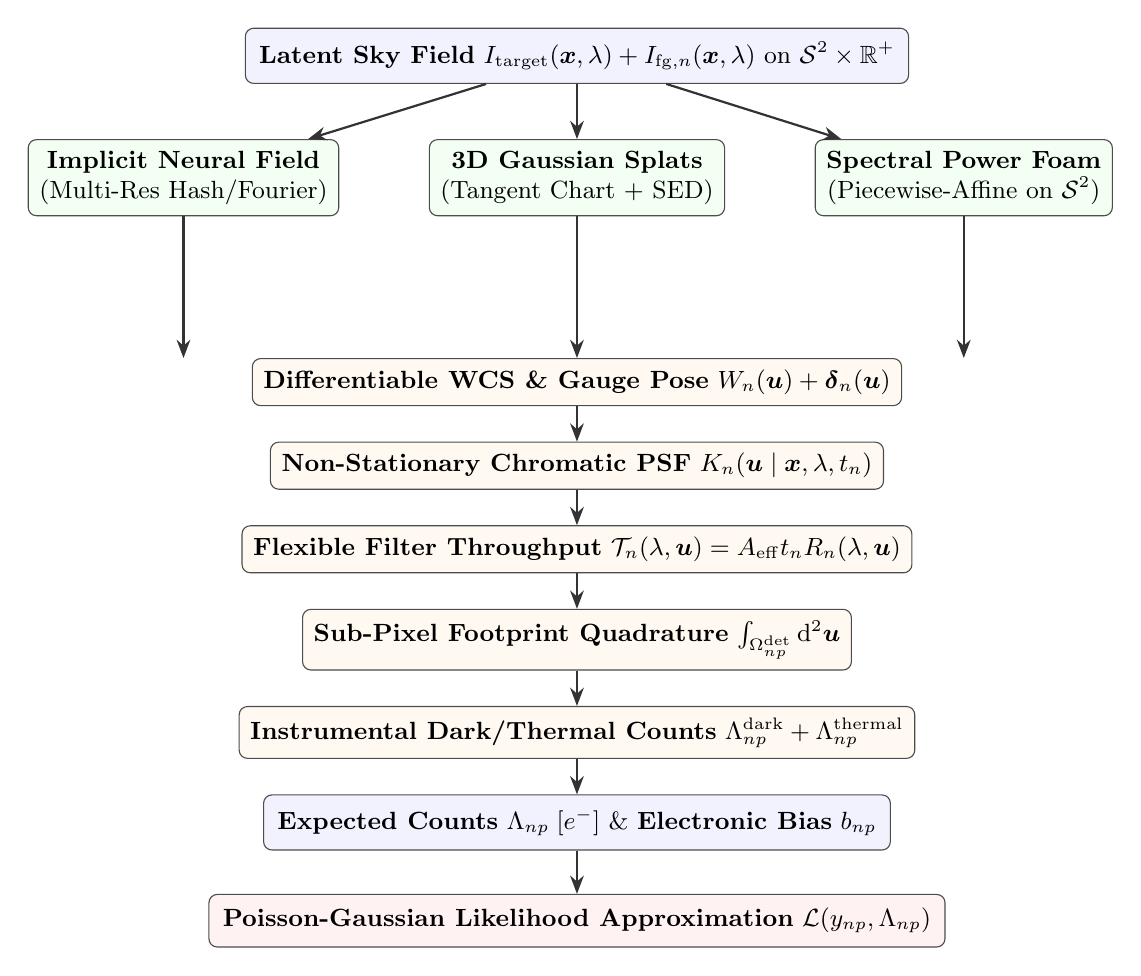
\begin{tikzpicture}[
    node distance=0.85cm and 0.5cm,
    box/.style={draw=black!70, rounded corners=3pt, fill=blue!5, align=center, font=\small, inner sep=5pt},
    repbox/.style={draw=black!70, rounded corners=3pt, fill=green!5, align=center, font=\small, inner sep=4pt},
    opbox/.style={draw=black!70, rounded corners=3pt, fill=orange!5, align=center, font=\small, inner sep=4pt},
    lossbox/.style={draw=black!70, rounded corners=3pt, fill=red!5, align=center, font=\small, inner sep=5pt},
    arrow/.style={-{Stealth[scale=1.0]}, thick, color=black!80}
]

\node[box] (sky) {\textbf{Latent Sky Field} $I_{\rm target}(\boldsymbol{x}, \lambda) + I_{{\rm fg}, n}(\boldsymbol{x}, \lambda)$ on $\mathcal{S}^2 \times \mathbb{R}^+$};

\node[repbox, below left=0.7cm and -1.2cm of sky] (inr) {\textbf{Implicit Neural Field}\\(Multi-Res Hash/Fourier)};
\node[repbox, below=0.7cm of sky] (splats) {\textbf{3D Gaussian Splats}\\(Tangent Chart + SED)};
\node[repbox, below right=0.7cm and -1.2cm of sky] (foam) {\textbf{Spectral Power Foam}\\(Piecewise-Affine on $\mathcal{S}^2$)};

\node[opbox, below=1.8cm of splats] (wcs) {\textbf{Differentiable WCS \& Gauge Pose} $W_n(\boldsymbol{u}) + \boldsymbol{\delta}_n(\boldsymbol{u})$};
\node[opbox, below=0.45cm of wcs] (psf) {\textbf{Non-Stationary Chromatic PSF} $K_n(\boldsymbol{u} \mid \boldsymbol{x}, \lambda, t_n)$};
\node[opbox, below=0.45cm of psf] (filter) {\textbf{Flexible Filter Throughput} $\mathcal{T}_n(\lambda, \boldsymbol{u}) = A_{\rm eff} t_n R_n(\lambda, \boldsymbol{u})$};
\node[opbox, below=0.45cm of filter] (integ) {\textbf{Sub-Pixel Footprint Quadrature} $\int_{\Omega_{np}^{\rm det}} \mathrm{d}^2\boldsymbol{u}$};
\node[opbox, below=0.45cm of integ] (bg) {\textbf{Instrumental Dark/Thermal Counts} $\Lambda_{np}^{\rm dark} + \Lambda_{np}^{\rm thermal}$};
\node[box, below=0.45cm of bg] (pixels) {\textbf{Expected Counts} $\Lambda_{np} \; [e^-]$ \& \textbf{Electronic Bias} $b_{np}$};
\node[lossbox, below=0.55cm of pixels] (loss) {\textbf{Poisson-Gaussian Likelihood Approximation} $\mathcal{L}(y_{np}, \Lambda_{np})$};

\draw[arrow] (sky) -- (inr);
\draw[arrow] (sky) -- (splats);
\draw[arrow] (sky) -- (foam);

\draw[arrow] (inr) -- (wcs.north -| inr);
\draw[arrow] (splats) -- (wcs);
\draw[arrow] (foam) -- (wcs.north -| foam);

\draw[arrow] (wcs) -- (psf);
\draw[arrow] (psf) -- (filter);
\draw[arrow] (filter) -- (integ);
\draw[arrow] (integ) -- (bg);
\draw[arrow] (bg) -- (pixels);
\draw[arrow] (pixels) -- (loss);

\end{tikzpicture}
\caption{Modular, differentiable forward observation pipeline in \texttt{torchsky}.}
\label{fig:pipeline}
\end{figure}

\subsection{Matrix-Free Linear Subsolvers in Iterative Optimization}
For fixed geometric representations (e.g., fixed-site Power Foams or linear Gaussian splat bases), the inner appearance subproblem solves the regularized normal equations:
\begin{equation}
\left( \sum_n \boldsymbol{F}_n^\top \boldsymbol{H}_n^\top \boldsymbol{W}_n \boldsymbol{H}_n \boldsymbol{F}_n + \gamma \boldsymbol{D}^\top \boldsymbol{D} \right) \boldsymbol{c} = \sum_n \boldsymbol{F}_n^\top \boldsymbol{H}_n^\top \boldsymbol{W}_n \boldsymbol{y}_n + \gamma \boldsymbol{D}^\top \boldsymbol{D} \boldsymbol{c}_0,
\end{equation}
solved matrix-free via Preconditioned Conjugate Gradients (Jacobi-PCG). For robust, heteroscedastic, or nonlinear objectives, this linear solve is embedded as the inner step of an outer Iteratively Reweighted Least Squares (IRLS) or Gauss-Newton framework.

\vspace{1em}
\hrule
\vspace{1em}

\section{Classical Baselines \& Rigorous Experimental Protocol}

\subsection{Comprehensive Comparator Matrix}
To prevent straw-man evaluations, learned continuous models are benchmarked against both classical coaddition pipelines and native-pixel un-resampled baselines, ensuring identical SED and source-family assumptions wherever feasible:
\begin{table}[htbp]
\centering
\small
\begin{tabularx}{\textwidth}{l p{5.5cm} X}
\toprule
\textbf{Pipeline / Family} & \textbf{Specific Configuration} & \textbf{Role in Benchmark} \\
\midrule
\textsc{Torchsky Stack} & Inverse-variance weighted bilinear/splat & Internal classical mapmaking control \\
Upstream \textsc{Drizzle} & \texttt{drizzlepac} square Drizzle ($\mathrm{pixfrac} \in \{0.6, 0.8, 1.0\}$) & Standard space-telescope (HST/JWST) comparator \\
\textsc{SWarp} & \textsc{SWarp} v2.41.5 (\texttt{BILINEAR} \& \texttt{LANCZOS3} with SIP$\to$TPV) & Standard ground/wide survey comparator \\
\textsc{Montage} & Area-weighted spherical polygon reprojection & Exact spherical geometry baseline \\
Whitened Multi-Band $\chi^2$ & Optimal matched filter over the best classical stacks & Strongest classical stack-level detection \\
\textbf{Native-Pixel GLRT} & Multi-band matched filter directly on all un-resampled exposures with matched SED/source prior & \textbf{Strongest native-pixel baseline}; isolates representation gains from stacking and prior effects \\
Linear Information Bound & Native-detector un-resampled Fisher linear estimate & Unbiased theoretical sensitivity reference \\
\bottomrule
\end{tabularx}
\caption{Comprehensive comparator matrix executed on identical calibrated detector inputs and permissible priors.}
\label{tab:baselines}
\end{table}

\subsection{Strict Protection Against the Inverse Crime}
To ensure that scientific depth gains are genuine and not artifacts of model self-consistency, \textbf{synthetic injections are strictly decoupled from the inference forward operator}:
\begin{itemize}
    \item \textbf{Independent Simulator for Truth Generation:} Injected truth sources are rendered using independent, physics-based optical wavefront simulators (e.g., \textsc{WebbPSF} utilizing measured optical path differences, pupil state models, and high-frequency jitter), empirical laboratory passbands with measured pupil angle variations, Gaia DR3 astrometric solutions, and realistic non-parametric galaxy morphologies from high-resolution HST/JWST cutouts.
    \item \textbf{Imperfect Inference Initialization:} The reconstruction engine initializes from nominal telescope models and must learn or fit residual calibrations without access to the simulator's internal truth parameters.
\end{itemize}

\subsection{Decoupled Validation Holdout vs.\ Full-Depth Science Evaluation}
We strictly separate predictive model validation from final depth measurement:
\begin{itemize}
    \item \textbf{Exposure Holdout (Predictive Generalization Gate):} Multi-dither exposures (e.g., JWST NIRCam SMACS J0723 in F090W, F150W, F200W, F277W, F356W, F444W) are split by dither pattern ($\mathrm{Train} = \{1, 2, 4, 5, 7\}$, $\mathrm{Val} = \{3, 8\}$, $\mathrm{Test} = \{6, 9\}$). This holdout is used exclusively to test out-of-fold predictive likelihood and verify that nuisance models do not overfit.
    \item \textbf{Full-Depth Science Evaluation:} Once hyperparameters and architecture are frozen, final scientific depth is measured using the complete exposure set across spatial-block cross-validation folds, matching real operational survey conditions.
\end{itemize}

\vspace{1em}
\hrule
\vspace{1em}
\section{Statistical Claim Gates \& Quantitative Metrics}
\label{sec:gates}

A reconstruction is scientifically certified as \emph{deeper} if and only if it satisfies all of the following pre-registered statistical gates:

\begin{enumerate}
    \item \textbf{Prevalence-Independent Completeness Depth.}\par
    The required inequality is $\Delta m_{50} > 0$.  Let $m_{50}$ be the
    reference-band AB magnitude at which the fitted source
    recovery probability is exactly $50\%$.  Evaluate it at a
    \textbf{fixed physical false-positive surface density},
    $\rho_{\rm false} \le \rho_0$ (for example,
    $\rho_{\rm false} \le 0.05\,\mathrm{arcmin^{-2}}$ on blank or null fields),
    thereby avoiding the prevalence dependence of sample-density purity:
    \begin{equation}
    \Delta m_{50} = m_{50}(\text{Continuous Latent Model}) - m_{50}(\text{Native-Pixel Baseline}).
    \end{equation}
    The paired $10{,}000$-sample cluster-bootstrap $95\%$ confidence interval for $\Delta m_{50}$ must strictly exclude zero.
    \item \textbf{Resolution-Matched Sensitivity Verification:}
    To prove that apparent variance reduction is not an artifact of prior over-smoothing or source broadening, we measure the 2D injection transfer function $\mathcal{H}_{\rm eff}(\boldsymbol{x})$ and effective PSF. Depth comparisons are evaluated at \textbf{matched effective spatial resolution}:
    \begin{equation}
    \sigma_{a, \rm eff} = \frac{\sqrt{\mathrm{Var}(\hat{a})}}{|R_a|} < \sigma_{a, \rm eff}^{\rm baseline} \quad \text{at matched spatial resolution}.
    \end{equation}
    \item \textbf{Photometric \& Color Invariants:}
    \begin{itemize}
        \item Bright point-source median absolute flux bias $\le 2\%$ per band.
        \item Adjacent-band median color bias $\le 0.02\,\mathrm{mag}$ across the smooth-continuum population.
    \end{itemize}
    \item \textbf{Population-Specific Expected Headroom Analysis:}
    Completeness curves $m_{50}$ must be reported separately across distinct astrophysical classes, reflecting their expected headroom hierarchy (isolated point sources $<$ extended sources $<$ blends / structured multi-band sources):
    \begin{itemize}
        \item \emph{Isolated Point Sources:} Limited headroom (heuristic working target $\Delta m_{50} \sim 0.05 - 0.2\,\mathrm{mag}$); the native-pixel GLRT is already near Neyman-Pearson optimal.
        \item \emph{Faint Extended Galaxies:} Moderate headroom (heuristic working target $\Delta m_{50} \sim 0.1 - 0.3\,\mathrm{mag}$); multi-exposure joint modeling beats rigid template matching.
        \item \emph{Crowded Blended Pairs ($\Delta \theta \le 1.5\,\mathrm{FWHM}$):} \textbf{High headroom}; multi-view chromatic deblending resolves sources lost to classical confusion.
        \item \emph{Extreme Dropouts ($z > 10$) \& Emission-Line Galaxies:} \textbf{High headroom}; joint cross-band evidence accumulation aggregates sub-threshold signals.
    \end{itemize}
    \item \textbf{Decisive Two-Stage Out-of-Sample Falsification Test (Held-Out Photon Prediction):}
    To conclusively distinguish genuine sensitivity improvements from prior-driven hallucinations, we enforce a two-stage discovery and confirmation protocol:
    \begin{enumerate}
        \item \emph{Discovery Reconstruction:} The model is fitted strictly on training exposures ($\mathrm{Train} = \{1, 2, 4, 5, 7\}$) to identify candidate sources discovered exclusively by the continuous method.
        \item \emph{Untouched Photon Prediction Test:} Candidate sources must statistically predict photon arrival patterns in untouched test exposures ($\mathrm{Test} = \{6, 9\}$) under the held-out likelihood-ratio statistic:
        \begin{equation}
        \Delta \log \mathcal{L}_{\rm heldout} = \log p(\boldsymbol{y}_{\rm test} \mid \hat{I}_{\rm candidate}) - \log p(\boldsymbol{y}_{\rm test} \mid I_{\rm no\text{-}candidate}) > \tau_{\rm null},
        \end{equation}
        where threshold $\tau_{\rm null}$ is calibrated on blank/null sky positions to control random false positives.
        \item \emph{Production Refit:} Only after confirmation are all exposures combined for final science products.
    \end{enumerate}
    \item \textbf{Spatial Homogeneity:}
    Depth gains must hold across at least two independent spatial quadrants, confirming that the improvement is not localized to a single favorable patch.
    \item \textbf{Model Selection on Validation Batches Only:}
    Every $(\text{scene kind}, \text{operator rung})$ cell of the model zoo (\S\ref{subsec:parameterizations}, \S\ref{subsec:hybrid_operators}) is scored on validation batches only ($\mathrm{Val} = \{3, 8\}$): $\Delta m_{50}$ with $10{,}000$-sample cluster-bootstrap CIs, matched-resolution $\sigma_{a,\rm eff}$, flux/color invariants, and held-out $\Delta\log\mathcal{L}$. The winning cell is the largest $\Delta m_{50}$ among cells passing all invariants; the untouched test exposures are scored exactly once after selection. A learned-PSF cell that fails the held-out-star NLL improvement gate is reported but cannot win unless it also beats the analytic arm's held-out gate.
\end{enumerate}

\vspace{1em}
\hrule
\vspace{1em}

\section{COSMOS Scale-Up Configuration}
\label{sec:cosmos}
The SMACS J0723 protocol generalizes mechanically to a wide-field survey target. The reference scale-up is \textbf{COSMOS}: a $2\,\mathrm{deg}^2$ field centered at $(\alpha, \delta) = (150.119^\circ, +2.205^\circ)$, combining:
\begin{itemize}
    \item \textbf{Space UV/Optical/IR:}
    JWST/NIRCam COSMOS-Web F115W, F150W, F277W, and F444W;
    JWST/MIRI F770W; and HST/ACS F606W and F814W.
    \item \textbf{Ground Optical:} Subaru/HSC $g\,r\,i\,z\,y$; CFHT/MegaCam $u^{*}$.
\end{itemize}
The field is partitioned into $0.25\,\mathrm{deg}^2$ tiles with $128$-pixel overlap; adjacent tiles are blended by a partition-of-unity weight so that each tile carries its own \texttt{FieldDomain} while global scene continuity is preserved across seams. Each instrument contributes an independent operator bundle: learned PSFs where calibration star density allows (NIRCam, ACS), analytic fitted kernels otherwise (ground-based seeing-dominated bands) --- the hybrid ladder of \S\ref{subsec:hybrid_operators} is precisely what makes heterogeneous multi-instrument inference tractable. All claim gates of \S\ref{sec:gates} are evaluated identically per tile.

\vspace{1em}
\hrule
\vspace{1em}

\section{Astrophysical Applications \& Discovery Potential}

The ability to recover continuous, joint spatial-spectral sky fields directly from native detector exposures unlocks major scientific capabilities:

\begin{itemize}
    \item \textbf{Cosmic Dawn \& High-Redshift Dropouts ($z > 10$):} Faint primeval galaxies near the detection limit exhibit steep Lyman-break spectral cutoffs. A joint continuous spatial-spectral model borrows signal across all red/NIR channels while preserving sharp spectral discontinuities, recovering candidates that fall below the $3\sigma$ threshold in individual classical stacks.
    \item \textbf{Strong Gravitational Lensing \& Extreme De-blending:} In rich cluster cores, highly magnified, distorted arclets are embedded within bright cluster galaxy light and diffuse intra-cluster light (ICL). Continuous representations decouple compact point-like knots from diffuse extended emission without pixelation artifacts.
    \item \textbf{Heterogeneous Multi-Observatory Synergy:}
    Co-model observations from disparate space and ground optical/infrared
    facilities, including HST, JWST, Euclid, Rubin LSST, and Roman.  Their
    distinct pixel grids, non-uniform PSFs, and dither strategies map into one
    physically consistent $(\alpha, \delta, \lambda)$ scene.
    \item \textbf{Discovery of Unmodeled Structure via Open Residuals:} Subtracting the forward-rendered model from native detector exposures yields calibrated \emph{open residual maps}, exposing moving solar system objects, rapid transients, extreme emission-line sources, or exotic diffuse structures that violate smooth continuum priors.
    \item \textbf{Foundation Models for Cosmology (\textsc{cosmodist}):} Directly interfaces with next-generation deep learning architectures, providing exact unit-sphere 3D WCS coordinate mappings and continuous multi-modal cutouts for generative cosmological field modeling and distributional conformal inference.
\end{itemize}

\end{document}
